\section{How the Replication Works}
\begin{figure}[htbp]
  \centering
  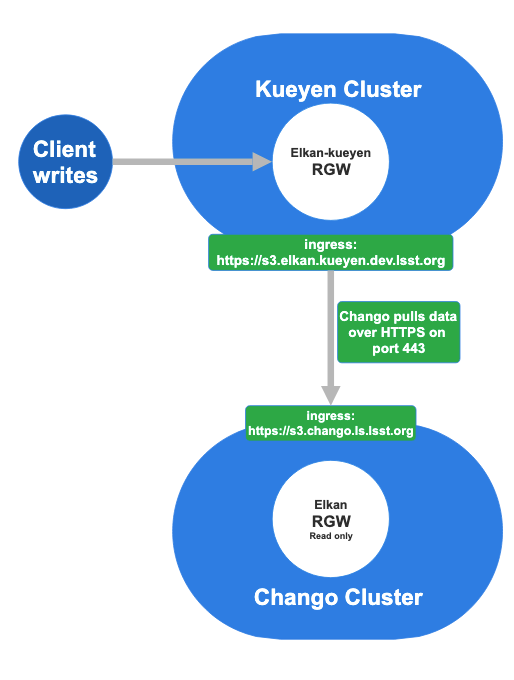
\includegraphics[width=0.8\textwidth,height=0.5\textheight,keepaspectratio]{Images/figure1.png}
  \caption{Replication flow from Elkan-Kueyen into Chango.}
\end{figure}

Figure 1 shows the replication flow. Clients and data producers write objects to the S3 endpoint of the source, which holds the master zone of the \texttt{elkan} realm. The source records each change in its RGW sync logs. Chango's read-only zone connects to the source endpoint over HTTPS, using the shared realm system keys, and pulls the realm configuration (period), the bucket and user metadata, and then the object data. Once replicated, the data stays on chango, which is the long-term storage location. The source only needs to hold data until it has been replicated. In the proof of concept, kueyen fills the source role, but any cluster or storage location configured as a master zone in the realm can do the same.
